\documentclass{beamer}

% Choose how your presentation looks.
%
% For more themes, color themes and font themes, see:
% http://deic.uab.es/~iblanes/beamer_gallery/index_by_theme.html
%
\mode<presentation>
{
  \usetheme{Darmstadt}      % or try Darmstadt, Madrid, Warsaw, ...
  \usecolortheme{beaver} % or try albatross, beaver, crane, ...
  \usefonttheme{serif}  % or try serif, structurebold, ...
  \setbeamertemplate{navigation symbols}{}
  \setbeamertemplate{caption}[numbered]
  \setbeamertemplate{footline}[frame number]
} 
\usepackage[english]{babel}
\usepackage[utf8]{inputenc}



\title[Progress Report]{Weekly Progress Report 5}
\author{Chloe Jamieson, Gabriel Garcia, and Ezra Decleene}
\institute{Bryan Summer Research Program\\ Advisor: Marilyn Vazquez \\ Simpson College}
\date{07/10/2026}

\begin{document}
\begin{frame}
  \titlepage
\end{frame}

\begin{frame}{Outline}
    \tableofcontents
\end{frame}

\section{Background}
\begin{frame}{Importance of the Biology}

\begin{itemize}
\item Spaceflight and microgravity can cause changes in human physiology
\item Directly studying these changes inside humans is difficult and highly invasive.
\item Tetrahymena are single-celled organisms with large numbers of cilia, making them a useful model for studying ciliary structure.
\end{itemize}

\end{frame}

\begin{frame}{Gravity Experiment}
    \begin{itemize} 
    
        \item Tetrahymena in normal gravity and microgravity
    
        \item Simulated gravity was created with a gyroscope
    \end{itemize}
        \centering
        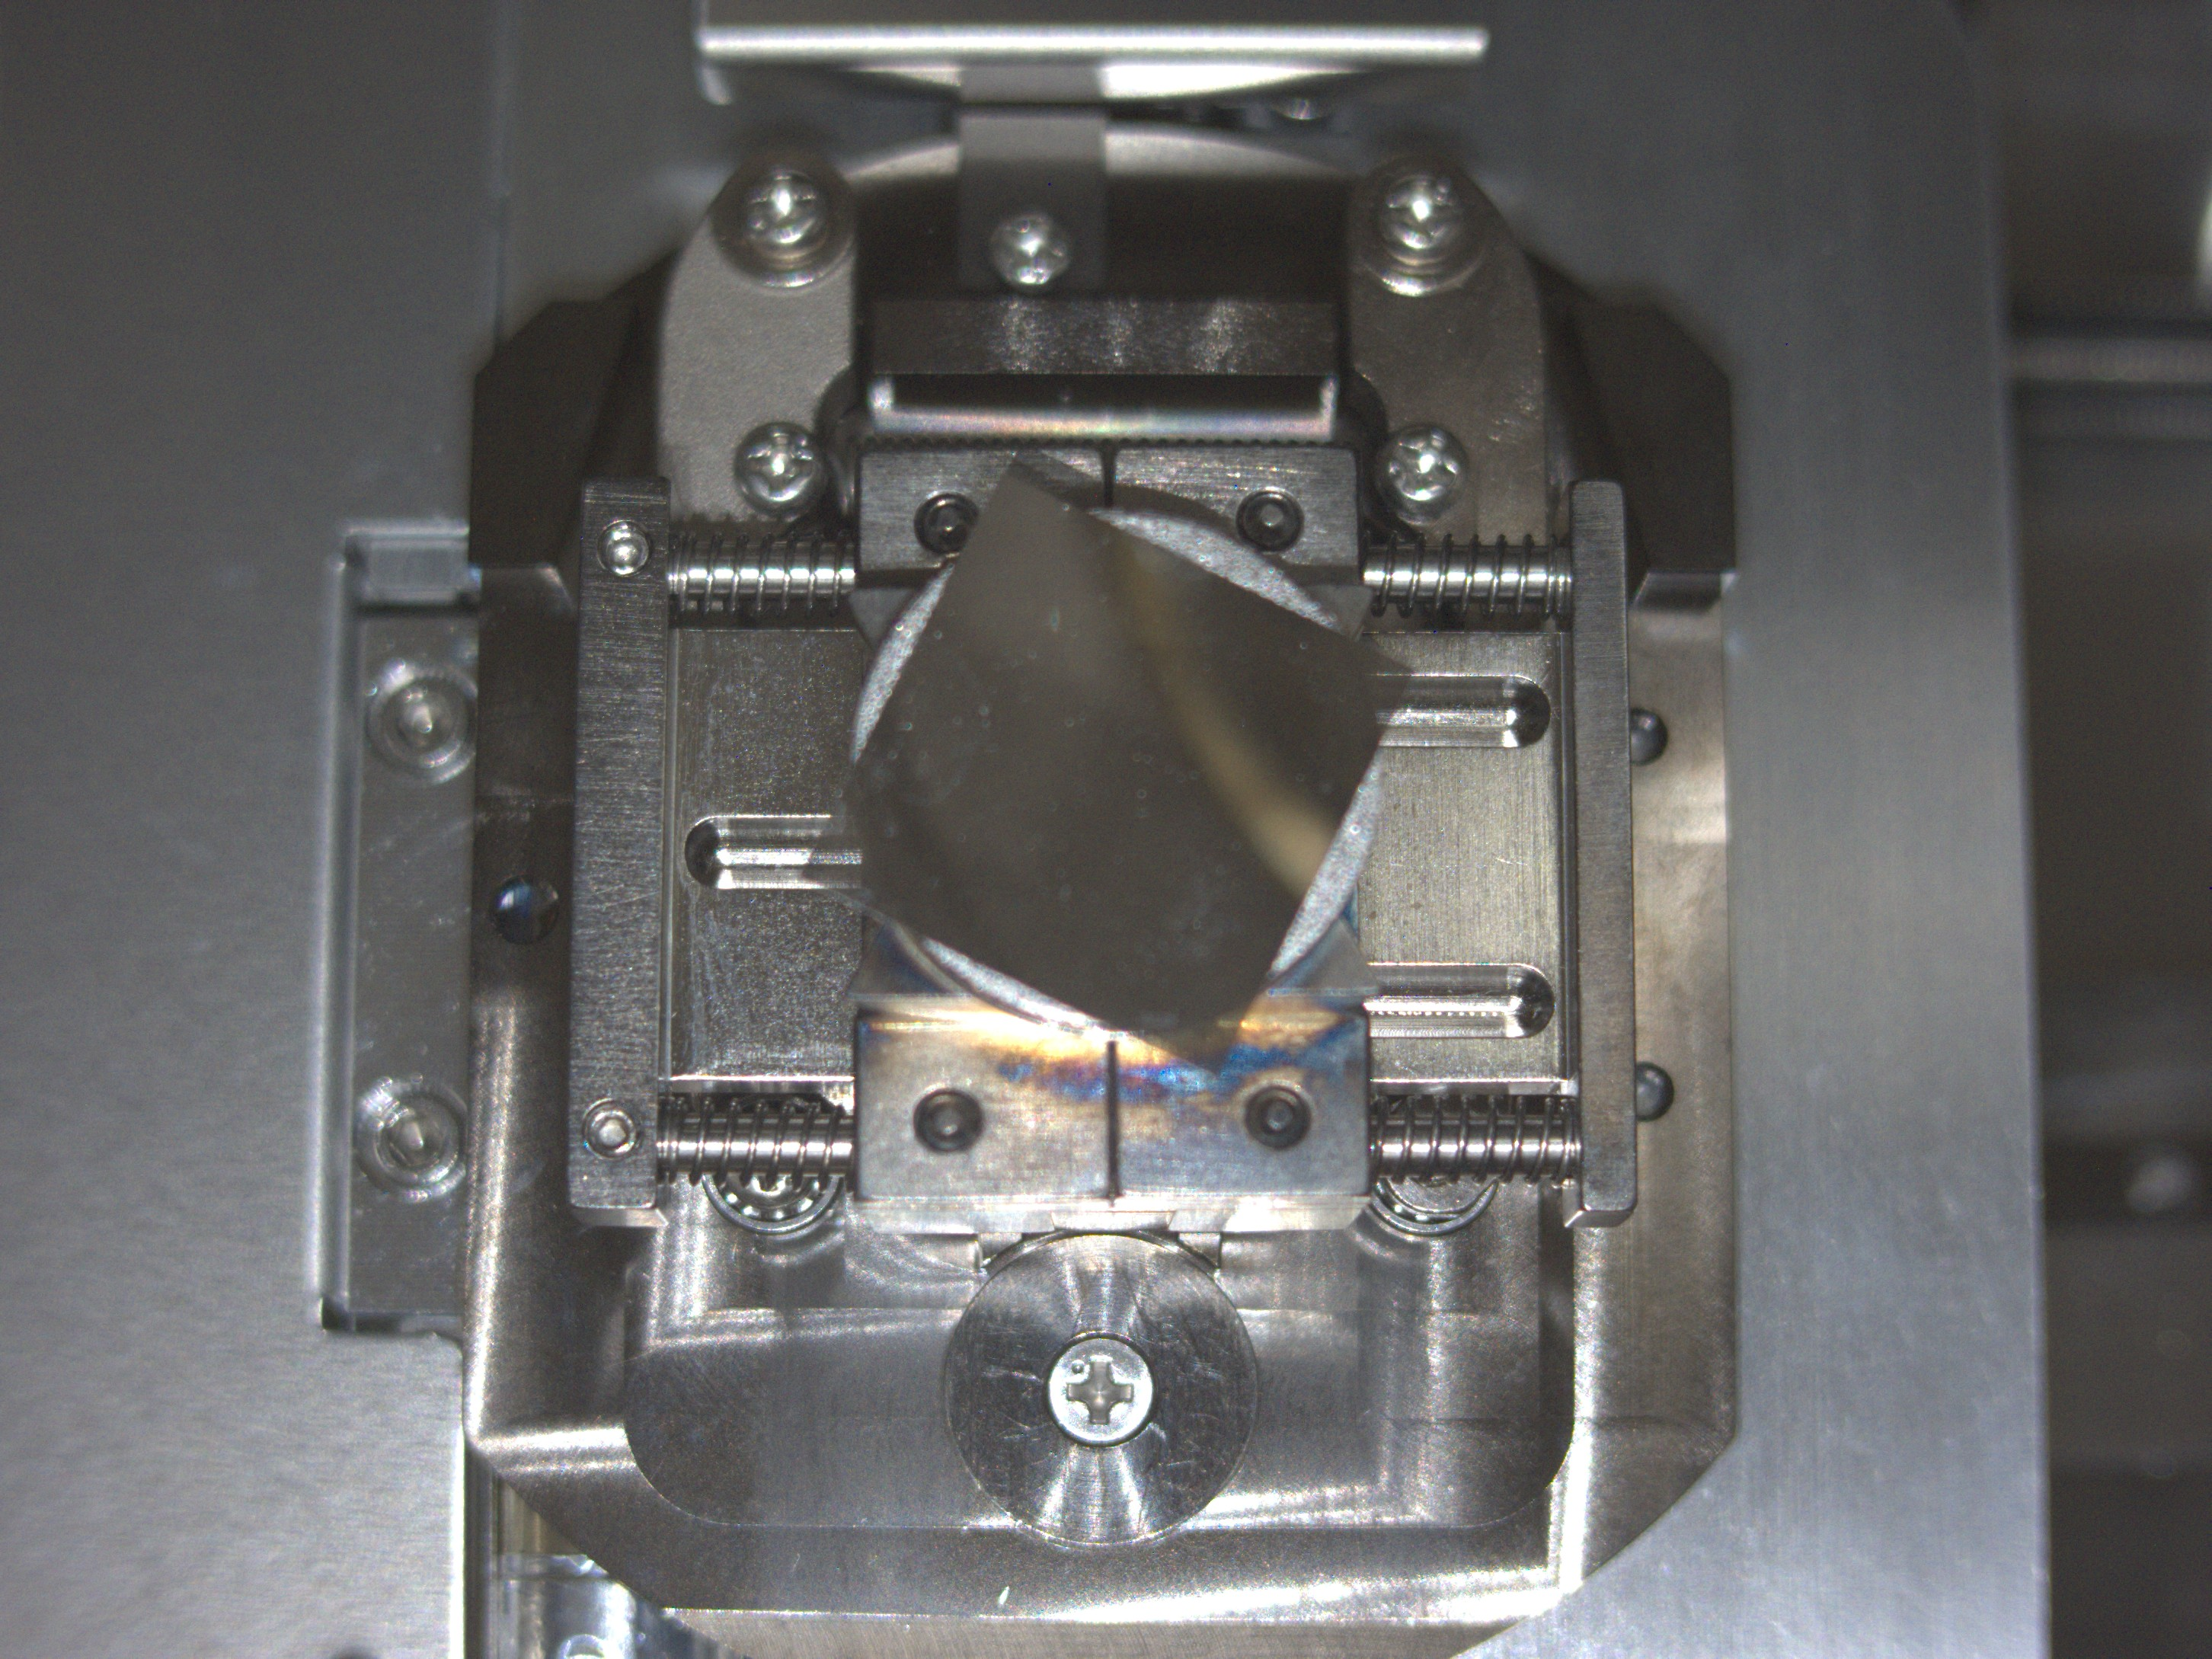
\includegraphics[height=0.6\textheight]{Images/Stub4C (1).jpg}

    
\end{frame} 

\begin{frame}{Why We Need Mathmateical Models}
\centering
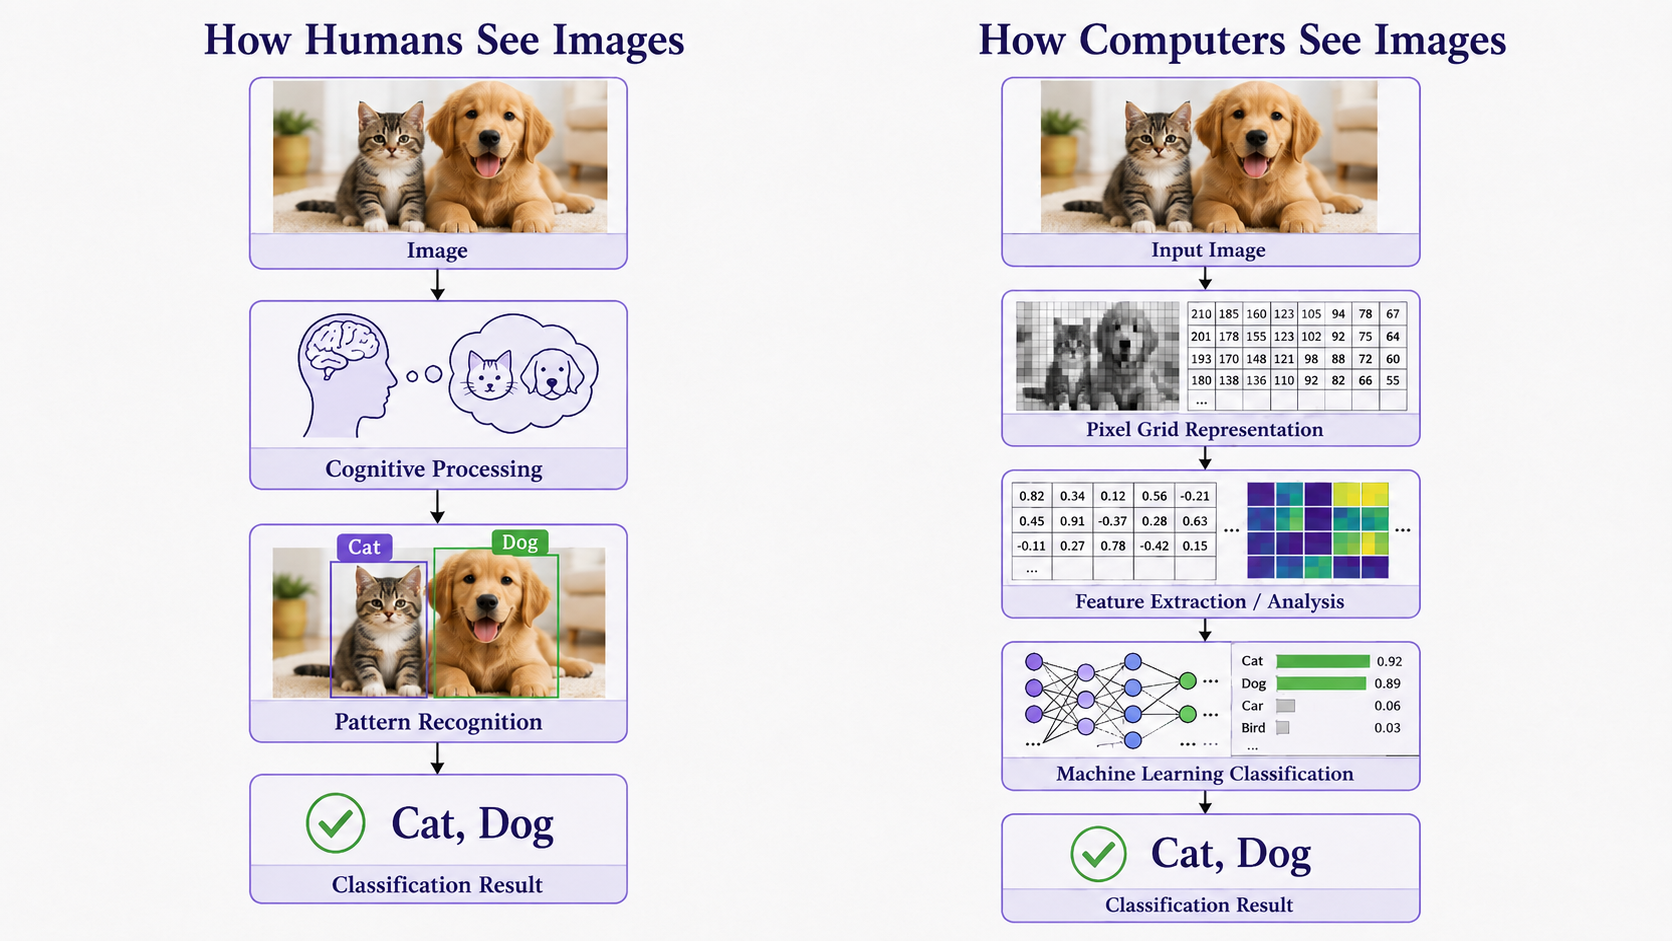
\includegraphics[width=\textwidth]{Images/HumanVsComputer.png}
\end{frame}

\begin{frame}{Goals}
\begin{itemize}
    \item Develop a pipeline to analyze cilia morphology using topological data analysis.
    \item Compare topological features from normal gravity and simulated microgravity images.
    \item Evaluate whether persistent homology can classify differences in cilia structure.
\end{itemize}
\end{frame}

\begin{frame}{Diagram}
    \centering
    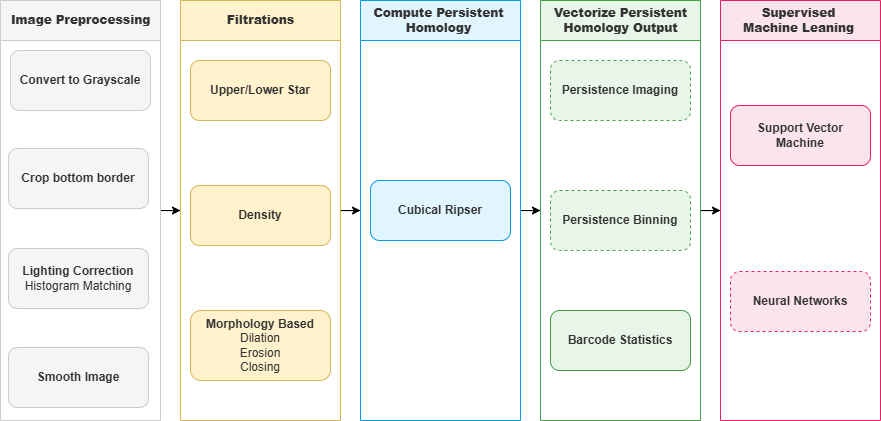
\includegraphics[width=1.\textwidth]{Images/Pipeline Diagramv2.drawio (1).png}
\end{frame}

\section{Preprocessing}
\begin{frame}{Why Preprocessing?} 
\begin{columns}[T] 
\begin{column}{0.48\textwidth} 
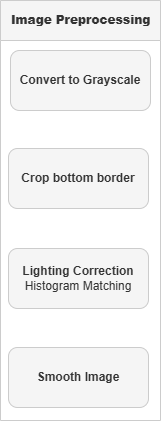
\includegraphics[width=0.5\textwidth]{Images/Image Preprocessing.png}
\end{column} 
\begin{column}{0.48\textwidth} 
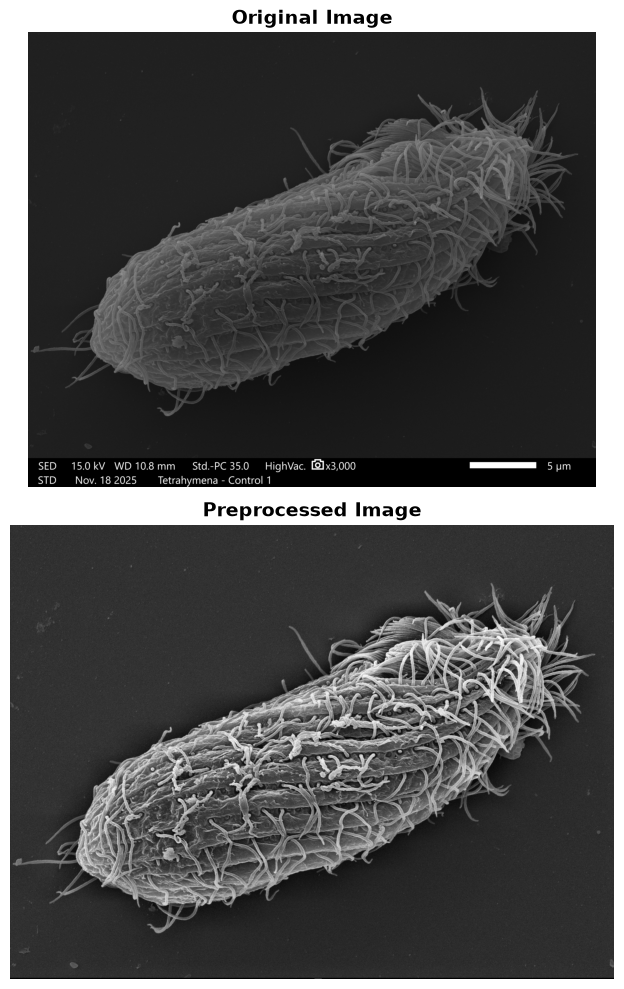
\includegraphics[width=0.75\textwidth]{Images/Figure 2026-07-09 154438.png} 
\end{column} 
\end{columns} 
\end{frame}




\section{Persistence}
\begin{frame}{Persistent Homology}

    % Left column
        \textbf{What does it do for us?}

        \vspace{0.3cm}

        \begin{itemize}
            \item Captures structural features in an image
            \item Measures how long structures persist as the image changes
            \item Produces a persistence diagram describing these features
        \end{itemize}

    % Right column
        \centering
        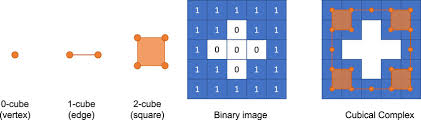
\includegraphics[
            width=\linewidth,
            height=0.65\textheight,
            keepaspectratio
        ]{Images/CubicalComplexExample.jpg}

\end{frame}

\begin{frame}{Filtration Methods}

\begin{columns}[T,onlytextwidth]

    % Left column
    \begin{column}{0.48\textwidth}
        We investigated several different filtration methods for persistent homology in image analysis. 
    \begin{itemize}
        \item \textbf{Intensity-based:} Lower Star / Upper Star
        \item \textbf{Shape-based:} Morphological Filtration
        \item \textbf{Density-based:} Density Filtration
\end{itemize}

        \vspace{0.3cm}

       
    \end{column}

    % Right column
    \begin{column}{0.48\textwidth}
        \centering

        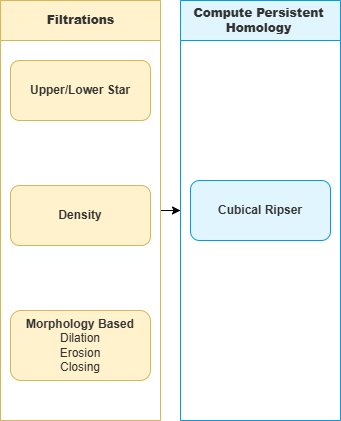
\includegraphics[
            width=\linewidth,
            height=0.65\textheight]{Images/PHandFiltrations.png}
    \end{column}

\end{columns}

\end{frame}

\begin{frame}{Lower/Upper Star}

    \begin{figure}
   \centering
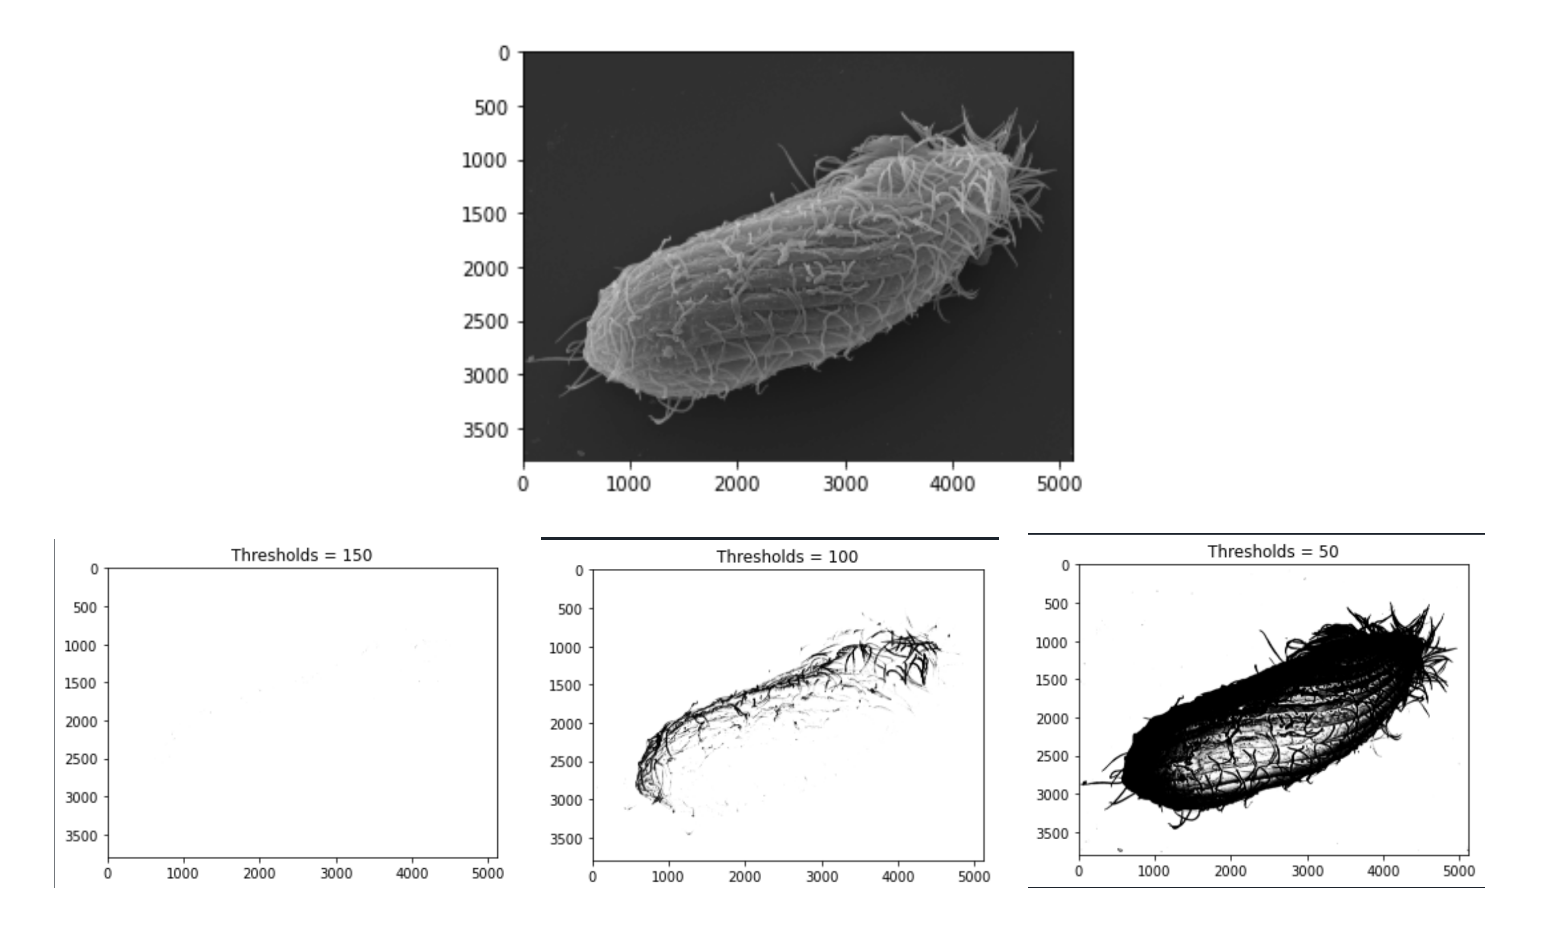
\includegraphics[width=\textwidth]{Images/Screenshot 2026-07-09 140553.png}
\end{figure}
\end{frame}

%\begin{frame}{Lower/Upper Star Persistence}
%    \begin{figure}
%    \centering
%\includegraphics[width=\textwidth]{Images/lowerandupper.png}
%\end{figure}
%\end{frame}

\begin{frame}{Morphology}
    \centering
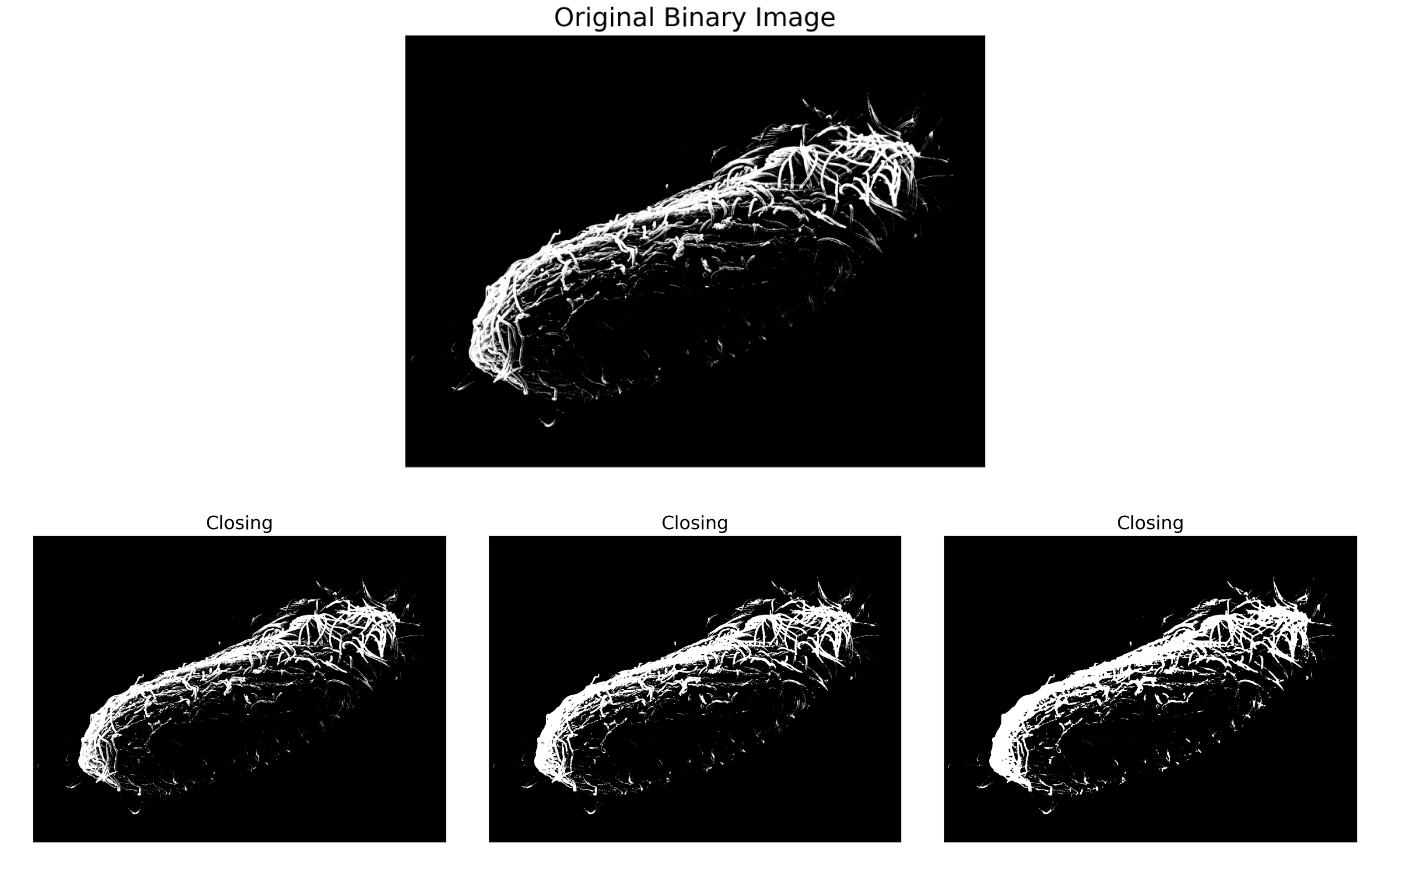
\includegraphics[width=\textwidth]{Images/Screenshot 2026-07-09 155736.png}
\end{frame}

\begin{frame}{Density}
 \centering
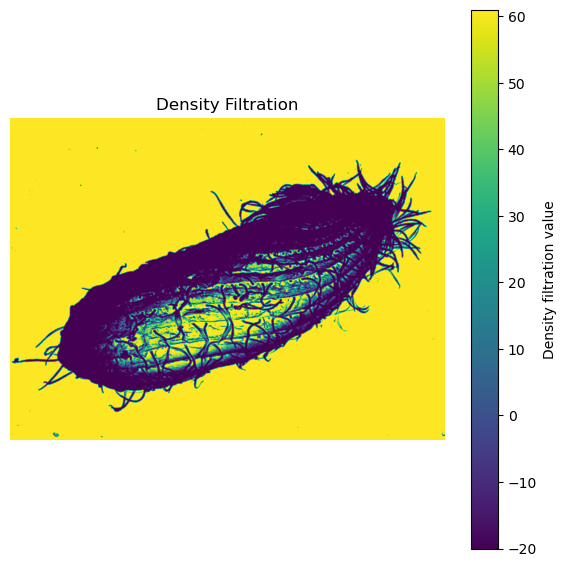
\includegraphics[width=.65\textwidth]{Images/Figure 2026-06-24 150818.png}
\end{frame}  

\section{Classification (Labeling)}

\begin{frame}{Vectorization}

\begin{columns}[T]

% Left column
\begin{column}{0.55\textwidth}

\textbf{Goal}
\begin{itemize}
    \item Convert persistence diagrams into numerical feature vectors for machine learning.
\end{itemize}

\vspace{0.3cm}

\textbf{Steps}
\begin{itemize}
    \item Compute persistence diagrams.
    \item Extract numerical features from each diagram.
    \item Create a fixed-length feature vector for each image.
\end{itemize}

\end{column}

% Right column
\begin{column}{0.40\textwidth}

\centering
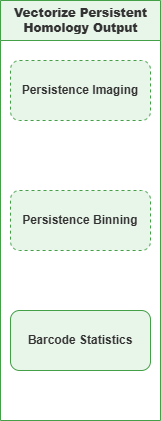
\includegraphics[width=.65\textwidth]{Images/Vectorization Diagram.png}

\end{column}

\end{columns}

\end{frame}
\begin{frame}{Vectorization: Barcode Statistics}
\centering
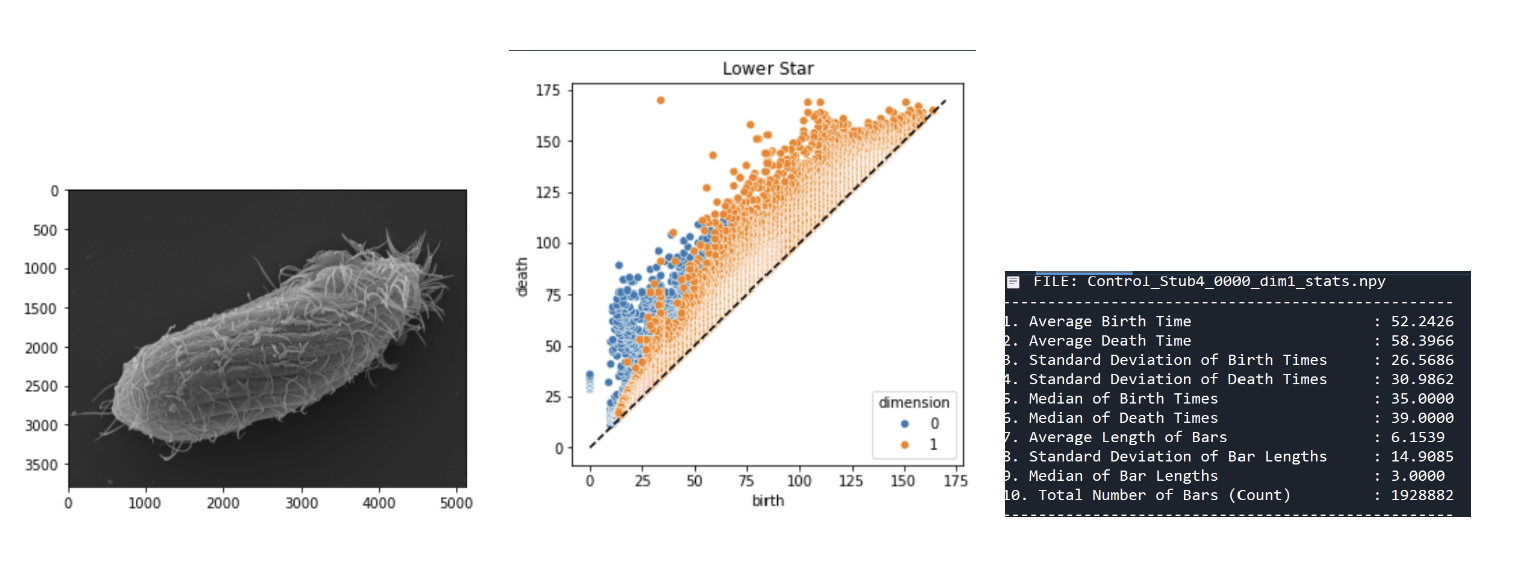
\includegraphics[width=\textwidth]{Images/Screenshot 2026-07-09 145027.png}

\end{frame} 

\begin{frame}{Vectorization: Binning}
    \begin{columns}[T]
\begin{column}{0.48\textwidth}
\begin{itemize}
    \item Rotates the persistence diagram to better represent feature persistence
    \item Divides the diagram into a fixed grid of bins
    \item Summarizes the persistence points that fall within each bin
    \item Flattens the bin values into a fixed-length vector for classification.
\end{itemize}
\end{column}

\begin{column}{0.48\textwidth}
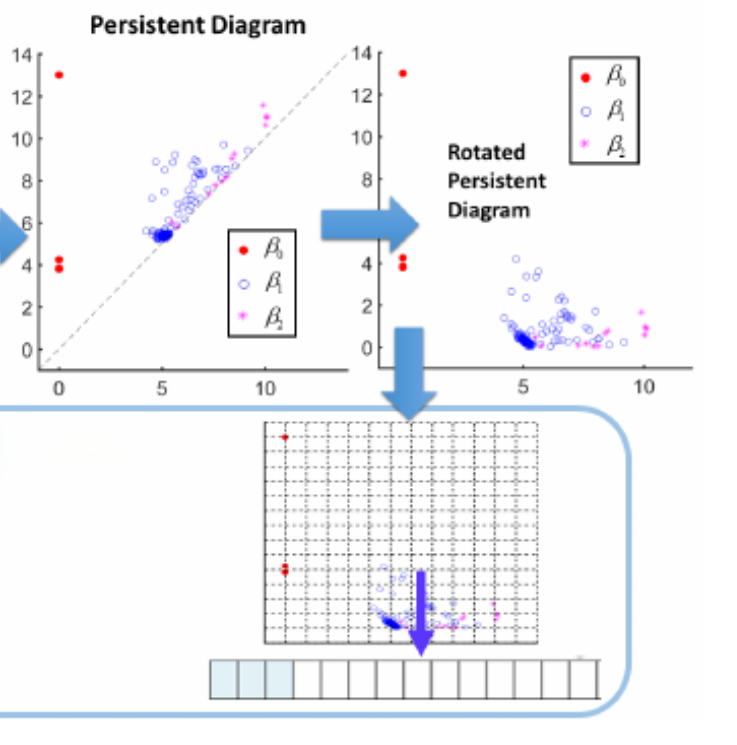
\includegraphics[width=\textwidth]{Images/Persistent Binning example.png}
\end{column}
\end{columns}
\end{frame}

\begin{frame}{Vectorization: Imaging}
    \centering

    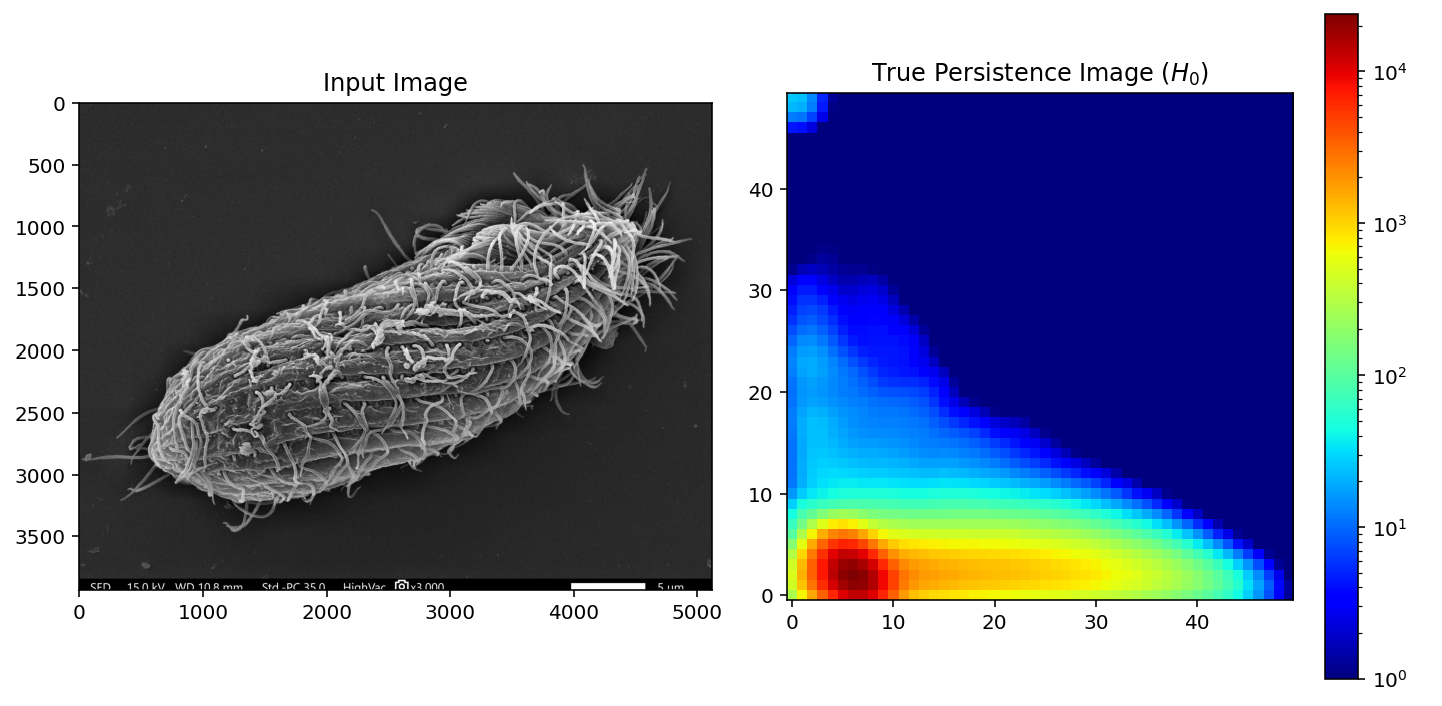
\includegraphics[width=0.65\textwidth]{Images/logimaging.png}

    \vspace{0.4cm}

    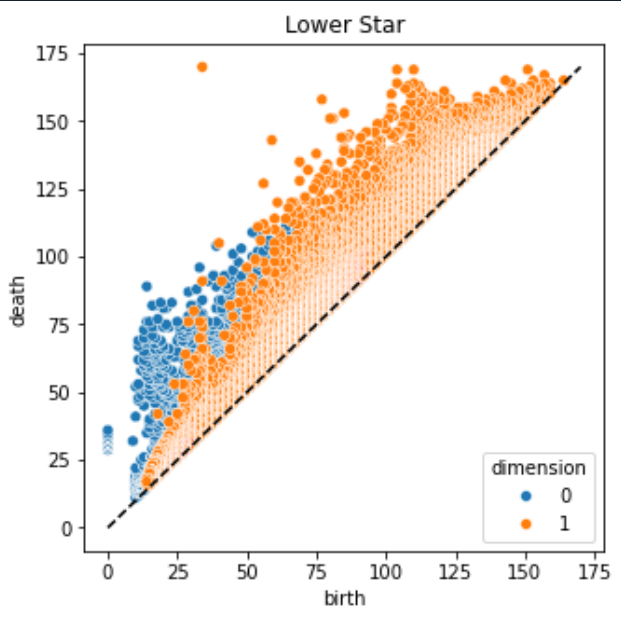
\includegraphics[width=0.35\textwidth]{Images/Screenshot 2026-06-10 153633.png}
\end{frame}



\begin{frame}{Support Vector Machines (SVM)}


\begin{columns}[T,onlytextwidth]

    % Left column
\begin{column}{0.48\textwidth}
    \textbf{Goal}
    \begin{itemize}
        \item Separate normal gravity and microgravity samples.
        \item Find the optimal decision boundary between classes.
    \end{itemize}

\vspace{0.3cm}

\textbf{Steps}
\begin{itemize}
    \item Input vectorized topological features.
    \item Train the SVM on labeled data.
    \item Classify unseen samples.
    \item Evaluate classification accuracy.
\end{itemize}

        \vspace{0.3cm}

       
    \end{column}

    % Right column
    \begin{column}{0.48\textwidth}
        \centering

        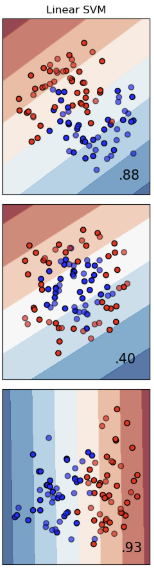
\includegraphics[
            width=0.5\linewidth,
            height=.75\textheight]{Images/Screenshot 2026-07-09 141641.png}
    \end{column}

\end{columns}
\end{frame}

\begin{frame}{Neural Networks}


\begin{columns}[T,onlytextwidth]

    % Left column
\begin{column}{0.48\textwidth}
    \textbf{Goal}
\begin{itemize}
    \item Learn complex patterns in topological features.
    \item Classify normal gravity and microgravity samples.
\end{itemize}

\vspace{0.3cm}

\textbf{Steps}
\begin{itemize}
    \item Input vectorized topological features.
    \item Train the network using labeled data.
    \item Adjust weights to minimize classification error.
\end{itemize}

        \vspace{0.3cm}

       
    \end{column}

    % Right column
    \begin{column}{0.48\textwidth}
        \centering

        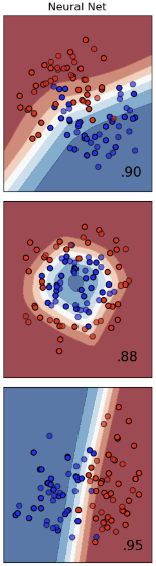
\includegraphics[
            width=0.5\linewidth,
            height=.75\textheight]{Images/Screenshot 2026-07-09 141652.png}
    \end{column}

\end{columns}


\end{frame}

\begin{frame}{Barcode Code Classifications}
\centering
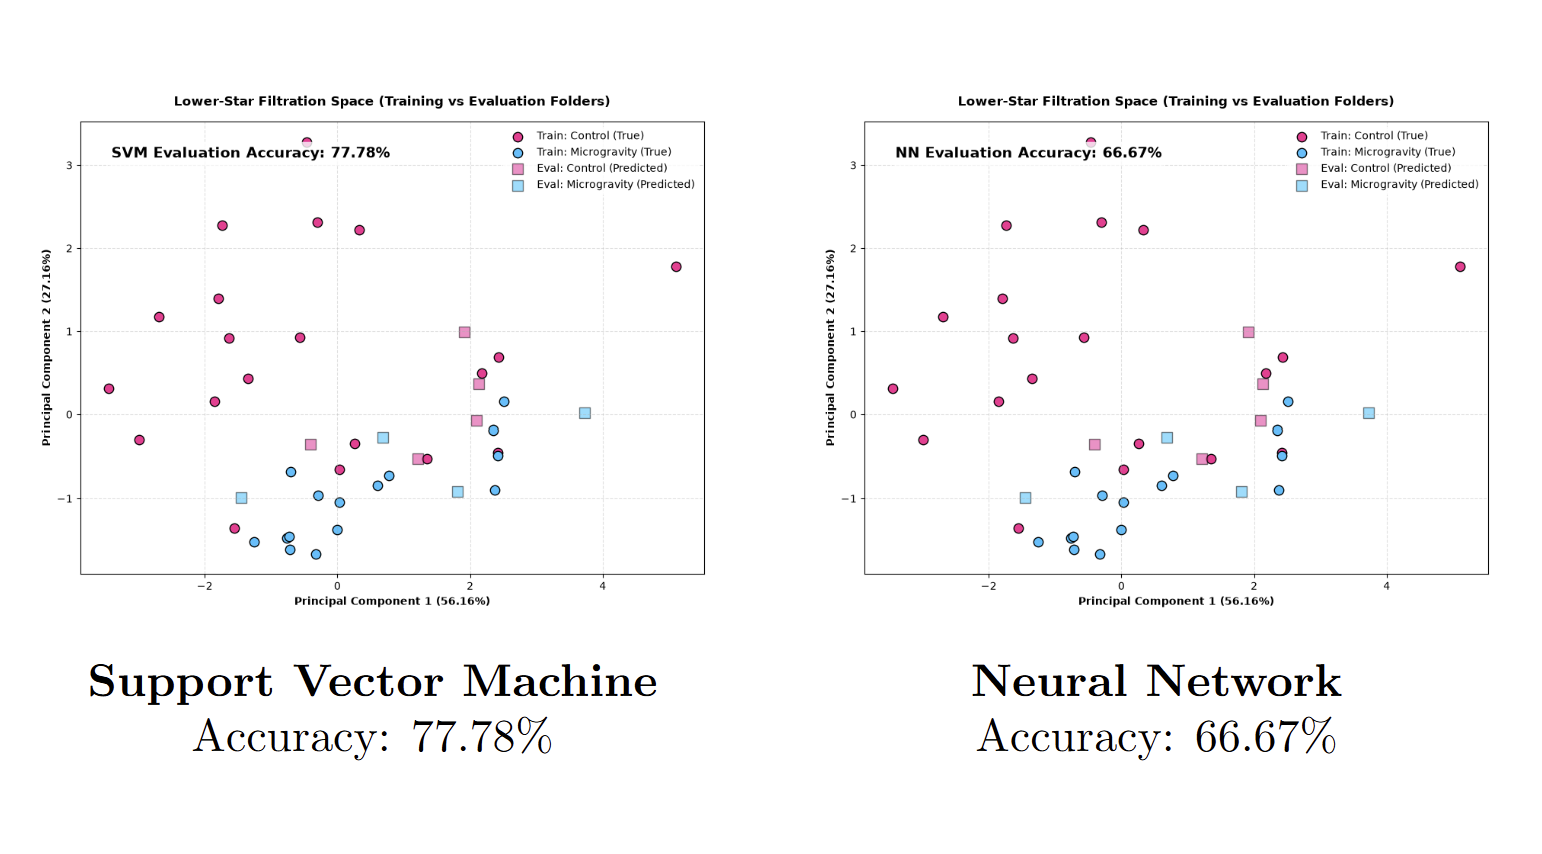
\includegraphics[width=\textwidth]{Images/Screenshot 2026-07-09 144410.png}
\end{frame}

\begin{frame}{Binning Classification}
\centering
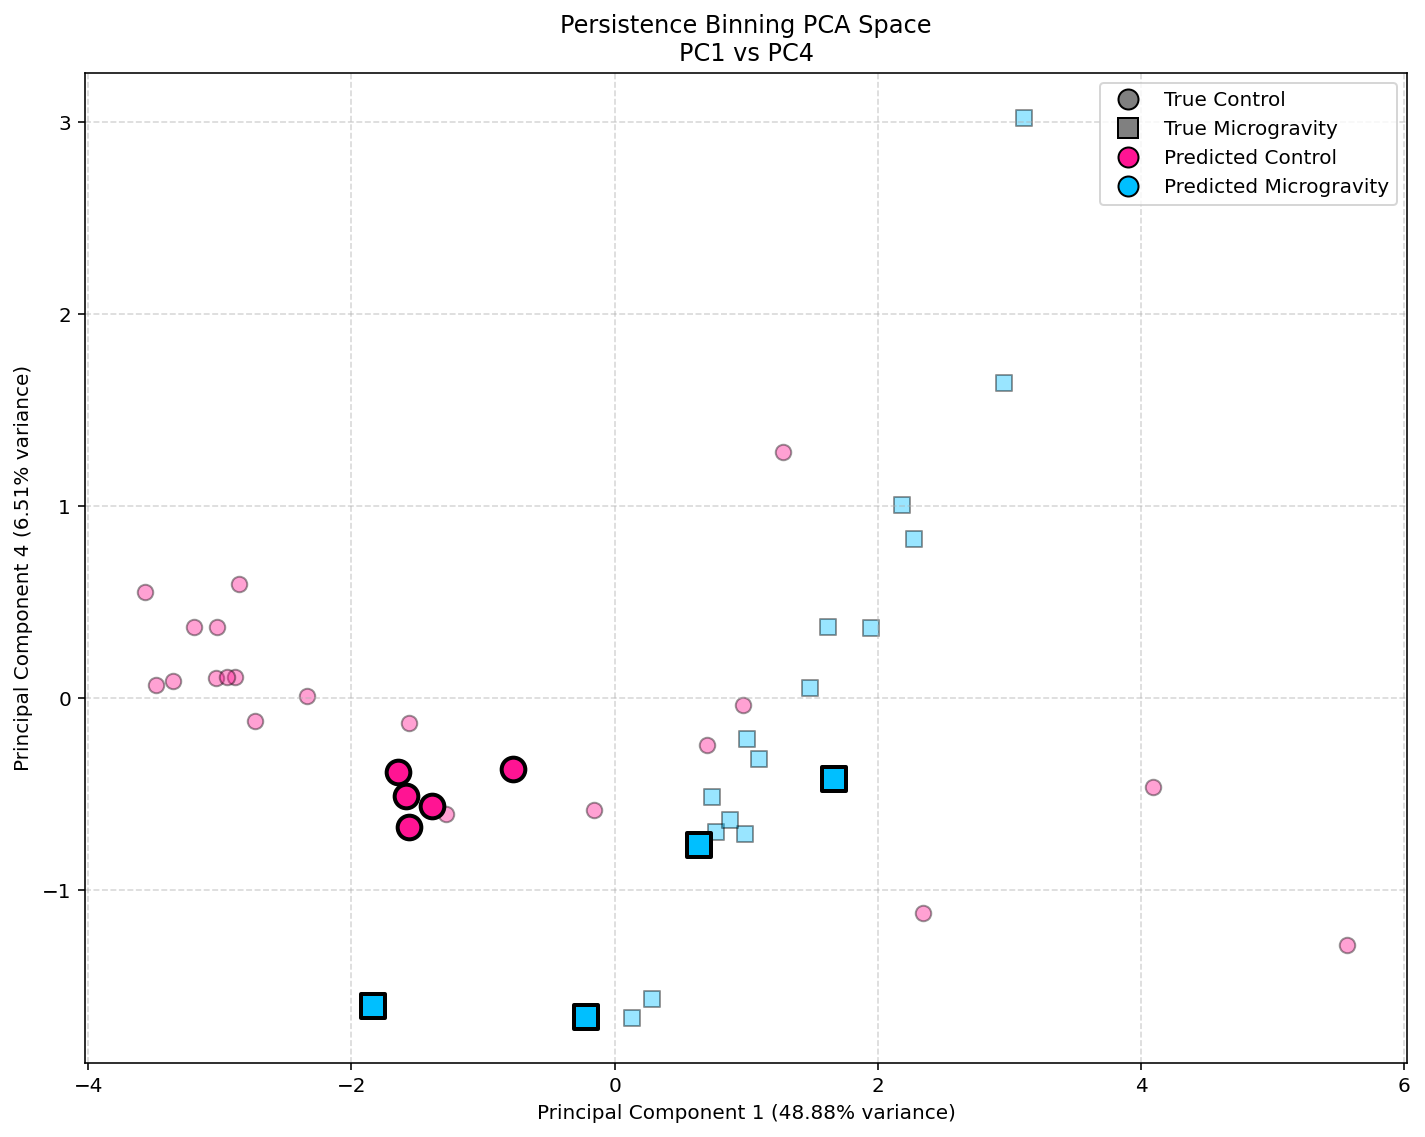
\includegraphics[width = 0.9\textwidth]{Images/svmBinning.png}
\end{frame}

\begin{frame}{Imaging Classification}
    \centering
    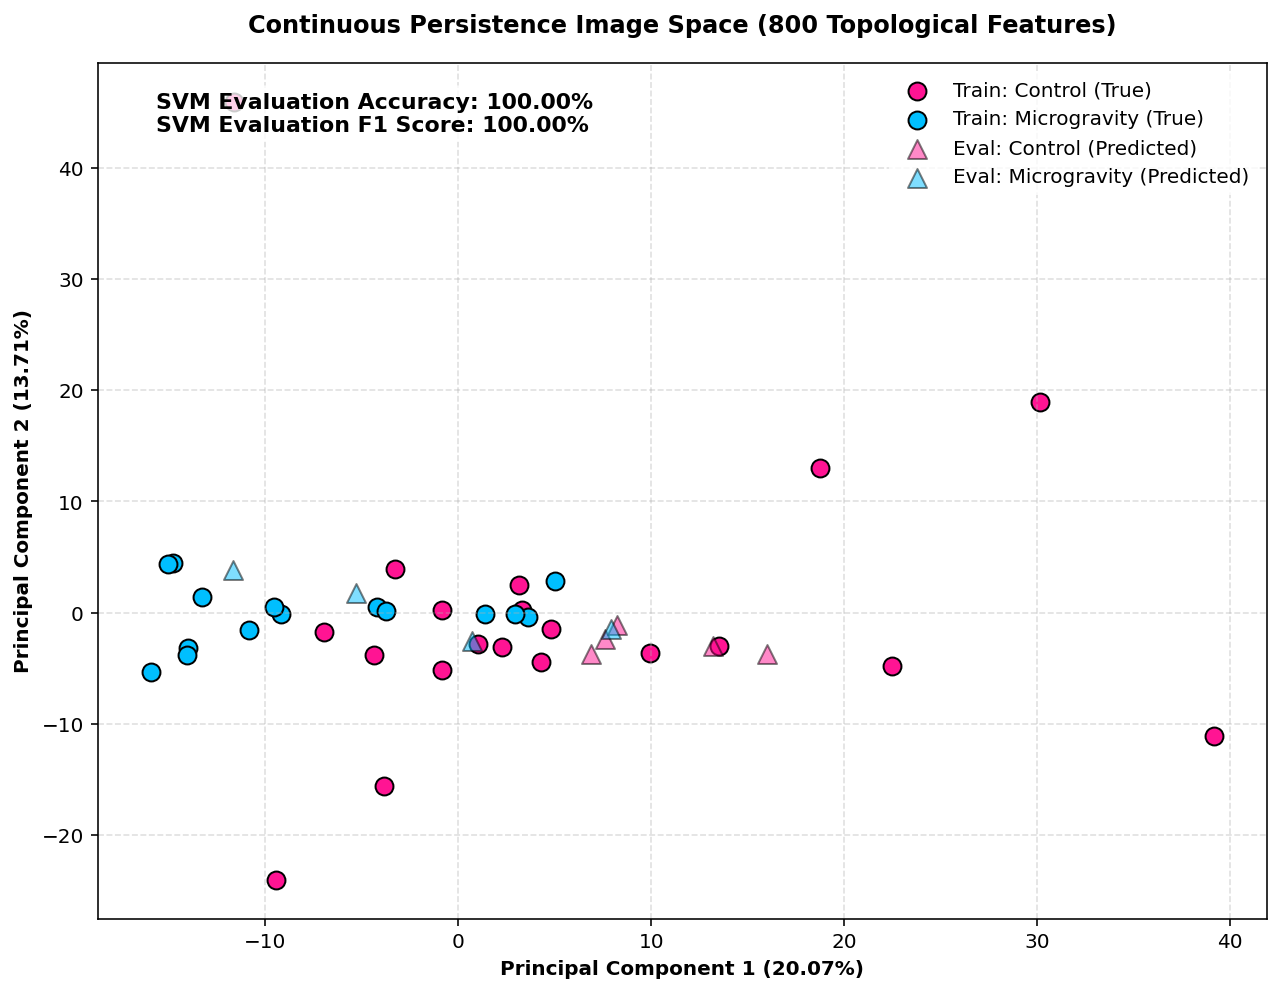
\includegraphics[width=0.9\textwidth]{Images/svmimaging.png}
\end{frame}

\section{Future Work}
\begin{frame}{Next Steps}
    \begin{itemize}
        \item Data Augmentation
        \begin{itemize}
            \item Due to the low amount of images we have, we'd like to create some more
            \item Involves rotating and shifting our current images
        \end{itemize}
        \item Verify that our classification results are accurate
        \begin{itemize}
            \item Shuffle around training and testing data to see if we get similar results
        \end{itemize}
        \item Use Neural Networks with Persistence Binning and Imaging
    \end{itemize}
\end{frame}


\section{Questions}
\begin{frame}
    \centering
    \vfill
    {\Huge Questions?}
    \vfill
\end{frame}

\end{document} 